\section{Visual Focus of Attention Estimation}
%Some kind of intro is needed here on why it is important to review the literature in this area.  It doesn't come across anywhere that this is a key technique you are using and why.
One of the key initiators of communication is joint attention, and grabbing and maintaining the visual attention of the user is an important functionality in the design of socially assistive robots \cite{torta2012can}.  In the context of this thesis, a robot is used to teach and practice hand-washing skills with children with ASD.  In its interaction with the child, successfully grabbing and maintaining the child's attention during the activity will ensure the child receives the prompts as the robot delivers it, and thus increasing the chance that the child complies to the prompts.  To this end, the robot behaviors need to be engaging to the child.  But more importantly, the robot behaviors should be contingent to the child's behaviors.  If the child is not paying attention, for example, an attention grabber (e.g. robot waves hand and call out to the child) would serve as a communication opener before delivering the prompt.  This enables the system to adhere to the DTT prompting framework mentioned in Section \ref{sec:DTTDiscussion}.  Because of this, the robotic system needs to be able to detect the visual attention of the child in real-time.

\subsection{Visual Focus of Attention and Gaze}
If we define Visual Focus of Attention (VFOA) as what a person is looking at, then given that we know what and where objects of interest are in the scene, the problem for VFOA estimation becomes estimating the direction and depth of a person's visual focus (i.e., gaze).
%Are there not standard definitions of these things that you can use and reference?

For consistency, we define the 3 degrees of freedom (DOFs) of head pose as pan, tilt, and roll (see Figure \ref{fig:murphy2009head}), with reference direction for pan and tilt being frontal direction of the head facing the camera.  We define 2 DOFs of eye pose as pan and tilt similar to head pose, with reference direction for pan and tilt same as head pose.
\begin{figure} [h]
	\centering
	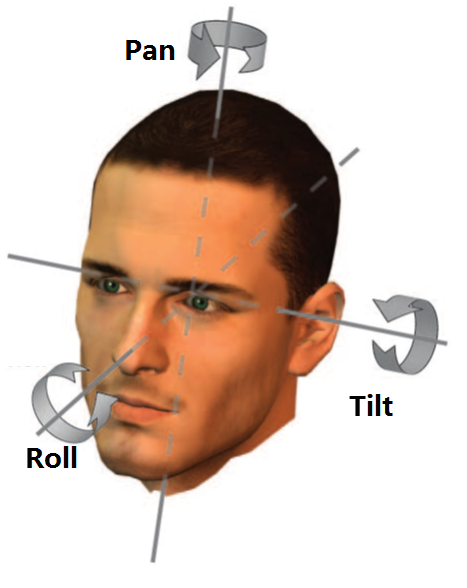
\includegraphics[width=0.6\textwidth]{./img/murphy2009head.png}
	\caption{DOFs of Head Pose, adapted from \cite{murphy2009head}}
	\label{fig:murphy2009head}
\end{figure}


Then, gaze direction is given by the accumulated rotation of average eye pose on head pose \cite{funes2013person}, gaze depth is given by the intersection of the left and right eye pose directions.  Therefore, the problem can be divided into head pose estimation and eye pose estimation.


\subsection{Head Pose Estimation}
There has been extensive research for head pose estimation for a single image frame, or head tracking for a video stream of images.  As reviewed by Murphy-Chutorian et al., the following categories of methods have been identified: appearance templates, detector arrays, nonlinear regression methods, manifold embedding methods, geometric methods, and flexible models \cite{murphy2009head}.


\subsubsection{Appearance Templates and Detector Arrays Methods}
Appearance templates methods and detector arrays methods are mainly for estimating discrete / coarse head pose.  For our task of identifying the object of interest under visual focus of attention, we do not know a priori where and how close to each other the objects are.  Therefore, only continuous fine pose estimation methods are of interest and are reviewed in this thesis.


\subsubsection{Nonlinear Regression Methods}
Using a machine learning approach, a direct mapping from the cropped head image to pose can be learned.  Because such mapping is highly nonlinear, nonlinear regression methods, such as Support Vector Regressors (SVR) \cite{li2000support} and Neural Networks (Multilayer Perceptron (MLP) \cite{voit2008head}, and Locally Linear Map (LLM) \cite{kruger2002gabor} have been applied in this context as supervised learning, using head images as inputs and head poses as ground truths.

Although neural networks are among the most popular and accurate methods in head pose estimation, they are prone to errors from poor head localizations.  And since, in our application, we cannot restrict user to remain in the center of the camera's field of view at all times, we need to either seek out a separate localization method for cropping the head, or seek a head tracker that doesn't have this problem.  Using face detectors for localization is one solution, but it only works for near frontal poses, bottlenecking the head tracker's operating range.


\subsubsection{Manifold Embedding Methods}
Manifold embedding methods learn a projection from high dimensional image space to some low dimensional space.  The methods are unsupervised learning methods that only require head images and not pose ground truth labels.  Promising techniques include: Isometric feature mapping (Isomap) \cite{raytchev2004head}, Locally Linear Embedding (LLE) \cite{roweis2000nonlinear}, and Laplacian Eigenmaps (LE) \cite{belkin2003laplacian}.


However, due to the fact that they ignore pose labels, the projected low dimensional space may not be capturing appearance variations due to head pose alone, but may also include appearance variations due to identity, lighting, etc., making pose prediction inaccurate.  Although there are work around techniques in the manifold embedding methods to tackle the appearance variations due to identity, more systematic ways to deal with it are seen in the following two methods: geometric methods and flexible model methods.


\subsubsection{Geometric Methods}
Geometric methods use person independent facial features (e.g. corners of eyes and mouth, tip of nose, etc.) to predict head pose.  The relative locations of these features are exploited with geometrical assumptions of a person's face such as parallelism, symmetry and proportion \cite{wang2007enhancement}.


A major caveat of these methods is that their accuracy relies on accuracy of features tracking.  For our scenario of a child washing hands at the sink, where a moderate resolution camera captures a mid-range field of view, features are not guaranteed to be tracked with ease.  Thus, it is better to select head pose estimation methods that do not require local features tracking.


\subsubsection{Flexible Model Methods}
Flexible model methods explicitly models the identity as well as pose of a person's face.  Given a representation of the face, flexible models for shape and texture can be constructed using PCA from a face database to represent the directions in which the face most likely (naturally) deforms.  Using this model, a new face image can be fitted through optimizing both an identity parameter and a pose parameter.  This way, pose can be extracted independent of identity.


There are two popular and related flexible model methods: Active Appearance Model (AAM) and 3D Morphable Model (3DMM).  They differ in the following ways:

\paragraph{Face Representation}
Although both models use triangulated mesh representations of the face, AAM uses a 2D representation while 3DMM uses a 3D one.  Also, AAM uses a sparse mesh with vertices at local features while 3DMM uses a dense mesh with vertices at the pixel level.  These make AAM more computationally efficient, but on the other hand 3DMM more robust to low resolution image, partial occlusions, lighting variations, and large head rotations.


\paragraph{Face Fitting}
Because AAM operates in 2D, fitting simultaneously the pose as well as the identity parameters requires us to recover a 3D model of the face using a structure-from-motion algorithm and then use the 3D model's weak perspective projection to constrain 2D fitting \cite{xiao2004real}.  3DMM fitting is less convoluted if using a RGB-D camera (e.g. the Kinect camera).  The pose and identity can be fit simultaneously using a non-rigid iterative closest point algorithm (Optimal Step Non-rigid ICP) \cite{paysan20093d}.

\subsubsection{Kinect Fusion}
Very similar to 3DMM, the Kinect Fusion algorithm developed by Microsoft also can be used to build a 3D head model, and track its orientation through ICP \cite{newcombe2011kinectfusion}.  The main difference between the two algorithms lies in that 3DMM uses the optimal step non-rigid ICP, which uses a parameterized model of a person's face generated by doing PCA of a face model database.  On the other hand, the head model generation from Kinect Fusion simply rely on building a point cloud of the head, thus its model is not parameterized.  Besides this head model generation step that is different, everything else used in head pose tracking are the same -- rigid ICP alignment.  However, since 3DMM focuses on modeling the face while Kinect Fusion is capable of modeling the whole head, Kinect Fusion may perform better in tracking extreme head poses where the face is largely obstructed.  3DMM, on the other hand, can be tolerant of dynamic expressions on a person's face \cite{amberg2008expression}, while Kinect Fusion may yield poorer tracking when the head model deforms.

\subsection{Eye Pose Estimation}
Eye pose estimation for a single image frame, or gaze tracking for video stream of images, have also been extensively researched.  Here we present results from a recent review by Hansen et al. \cite{hansen2010eye}.  Eye pose estimation methods can be categorized as shape-based, feature-based, and appearance-based:


\subsubsection{Shape-Based Methods}
Shape-based methods are seeking to contour fit the shapes of iris, pupil, eye, etc.  Some examples include: a simple model of ellipse fitting the shape of iris or pupil region, proposed by Valenti et al. \cite{valenti2008accurate}; a complex model of deformable template fitting the eye and pupil shape, proposed by Colombo et al. \cite{colombo1999real}.


\subsubsection{Feature-Based Shape Methods}
Feature-based shape methods seek eye structure localization through identifying a set of distinctive local features.  One can use features directly in the intensity image, with features found for example in limbus, pupil, cornea reflections, eye corners, etc.  An example for this is the neural network method by Reinders et al. \cite{reinders1996locating}.  One can also use features in a filter response of the image, for example seen in the method of A Sirohey et al. \cite{sirohey2001eye}.


Both the shape-based and feature-based methods are inaccurate for moderate resolution mid-range field of view images -- they often require a close up view of an eye.  The problem with large field of view containing not only the eye regions is two fold.  First, lower resolution for the eye regions are available, making the above methods less accurate.  Second, without a proper localization of the eyes, false positives arise.  Methods combining head pose and eye pose estimation is an effective way to combat the false positives in a large field of view as well as dealing with large head poses.  It improves accuracy through the two estimators constraining each other in localizations \cite{valenti2012combining}.  However, a better way, as seen in the head pose tracking section of the literature review, is to use appearance-based methods.


\subsubsection{Appearance-Based Methods}
Another approach to deal with moderate resolution mid-field images is through appearance-based methods.  One can directly model the mapping from eye appearance to eye pose, seen by the neural network method of Baluja et al. \cite{baluja1994non}.  However, direct modeling requires large number of training images, the collection of which is a tedious process.  One way to reduce number of training images needed is through template matching with local linear interpolation.  An example of this is the Adaptive Linear Regression (ALR) method of Lu et al. \cite{lu2011inferring}.


The major caveat with these appearance-based methods, as similarly to head pose estimation, is the inability to separate appearance variations in identity from pose.  One way to tackle this is through keeping a bank of personal models, seen in Mora et al. \cite{funes2013person}.  A new person's eye images can then be represented by a linear combination of exemplar eye images from people in the bank using ALR.  Then, to ease computational cost of ALR, we only keep the top few models that have their exemplar eye images used most often, decreasing the search space during ALR's optimization step.


\subsection{Using RGB-D Camera for Gaze Estimation}
The works of Mora et al. are good fits to our application \cite{funes2012gaze, funes2013person}.  Specifically, their approach uses the 3DMM head pose estimation together with ALR eye pose estimation.  One thing to note is that the commercial grade RGB-D camera, Kinect, is used.  Although 3DMM works with 2D camera as well, getting a direct sensor input on the depth information is advantageous in this context because it avoids inferring the 3D structure from 2D images, reducing inaccuracies and computations. Also, it enables 3DMM to estimate pose through shape alone, ignoring texture fitting altogether, reducing computations and increasing robustness to lighting.


\subsection{Discussion}
From the reviews, we see that Kinect Fusion and ALR are ideal for our application.  They yield many advantages:  Firstly, usage of appearance-based methods means we are moderate resolution mid-field scenario ready.  Secondly, only a simple calibration step is needed to generate the head model for Kinect Fusion and a bank of people's exemplar eye images are needed for ALR.  For the children with ASD population, having relatively simple calibration step that does not require the child to behave in a certain way is very useful.  Next, once the person's head model is generated, pose can be fitted without fitting identity, reducing computations.  Lastly, the head image can be restored to the frontal head pose and a consistent frontal eye region cropped out, making eye pose estimation robust to large head poses.
